\section{Luồng feedback câu trả lời để cải thiện chatbot}

Luồng feedback mô tả cách người dùng hoặc quản trị viên đánh giá chất lượng một câu trả lời, từ đó tạo ra dữ liệu đầu vào cho việc hiệu chỉnh rule, intent hoặc tài liệu ngữ cảnh. Đây là luồng rất quan trọng đối với một hệ thống học hỏi từ vận hành thực tế, vì nó biến phản hồi người dùng thành dữ liệu cải tiến có cấu trúc.

\begin{figure}[H]
    \centering
    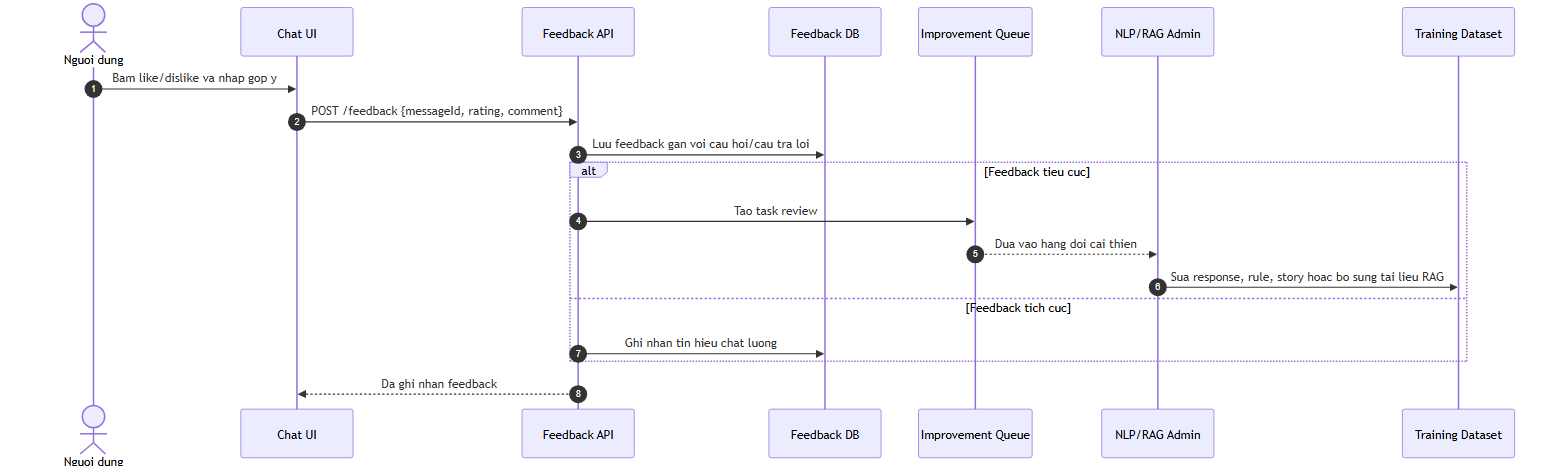
\includegraphics[width=\textwidth]{content/source/mermaid_sequence/seq_10.png}
    \caption{Luồng feedback câu trả lời để cải thiện chatbot}
\end{figure}

Về nghiệp vụ, sau khi chatbot trả lời, người dùng có thể đánh giá câu trả lời là phù hợp hoặc chưa phù hợp; thông tin này được gửi về backend và liên kết với câu hỏi, câu trả lời, ngữ cảnh hội thoại hoặc tài liệu tham chiếu đã sử dụng. Quản trị viên sau đó xem xét feedback, xác định nguyên nhân đến từ dữ liệu NLU, rule hội thoại hay truy xuất RAG, rồi cập nhật thành phần tương ứng. Luồng này là cầu nối giữa lớp sử dụng thực tế và lớp cải tiến chất lượng hệ thống.
